\documentclass[12pt]{report}

% General includes
\usepackage{amsfonts, amssymb, amsmath}
\usepackage{graphicx}
\usepackage{float}
\usepackage{color, soul}
\usepackage{hyperref}

% Font settings
%\renewcommand\familydefault{\sfdefault}
\usepackage{palatino}  % serif
\usepackage{helvet}    % sans-serif
\usepackage{courier}   % typewriter
\usepackage{euler}     % math mode

% Margin and paragraph indent
\usepackage[margin=1.0in]{geometry}
\usepackage{parskip}

%\geometry{paperwidth=30cm}
%\geometry{paperheight=40cm}


\begin{document}
\begin{titlepage}
	\centering
	\vspace{1cm}
	{\scshape\Large ESE 370: Circuit-Level Optimization for Digital Systems\par}
	\vspace{1.5cm}
	{\huge\bfseries Project 2 Milestone: FIFO Queue\par}
	\vspace{2cm}
	{\Large\itshape Mauricio Mutai, Jack Harkins\par}
	\vfill
	Instructor: Dr. Tania Khanna\par
	TA: Martin Deng\par
	Date: 11/26/16

	\vfill

% Bottom of the page
	{\large \today\par}
\end{titlepage}

\section*{Bitline Capacitance}
Each SRAM cell loads each bitline with a capacitance of $4\gamma C_0$. This can be seen in Figure \ref{fig:sram_cell_circuit} below, which shows that $BL$ and $BL'$ are each connected to the drain/source terminal of a transistor of width 4.

Next, each bitline is loaded with at most 16 SRAM cells. This number could be reduced by arranging the words in a 4x4 pattern, for example, but we will consider the worst case capacitance, which arises with 16 cells. Thus, each bitline is loaded with $64\gamma C_0$ from the SRAM cells.

In addition, each bitline is loaded with $16\gamma C_0$ from the driver circuit, and $16\gamma C_0$ from the tri-state buffer or inverter. Therefore, the total load on the bitline is $96\gamma C_0$.

\section*{Circuit Schematics}
\subsection*{Memory Column Driver Schematic}
\begin{figure}[H]
  \centering
    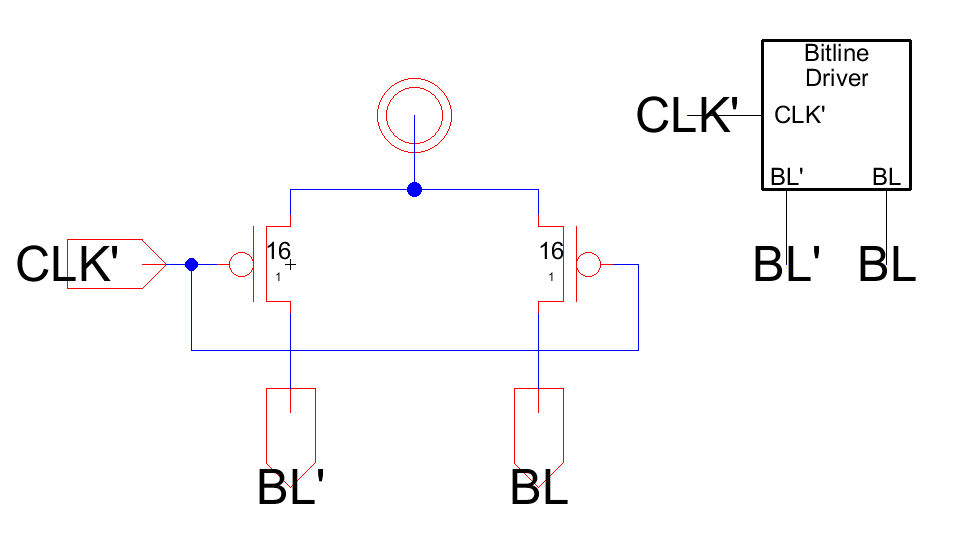
\includegraphics[width=1.0\textwidth]{bitline_driver_circuit.PNG}
  \caption{Bitline driver circuit}
  \label{fig:bitline_driver_circuit}
\end{figure}

\subsection*{Sized Memory Cell Schematic}
\begin{figure}[H]
  \centering
    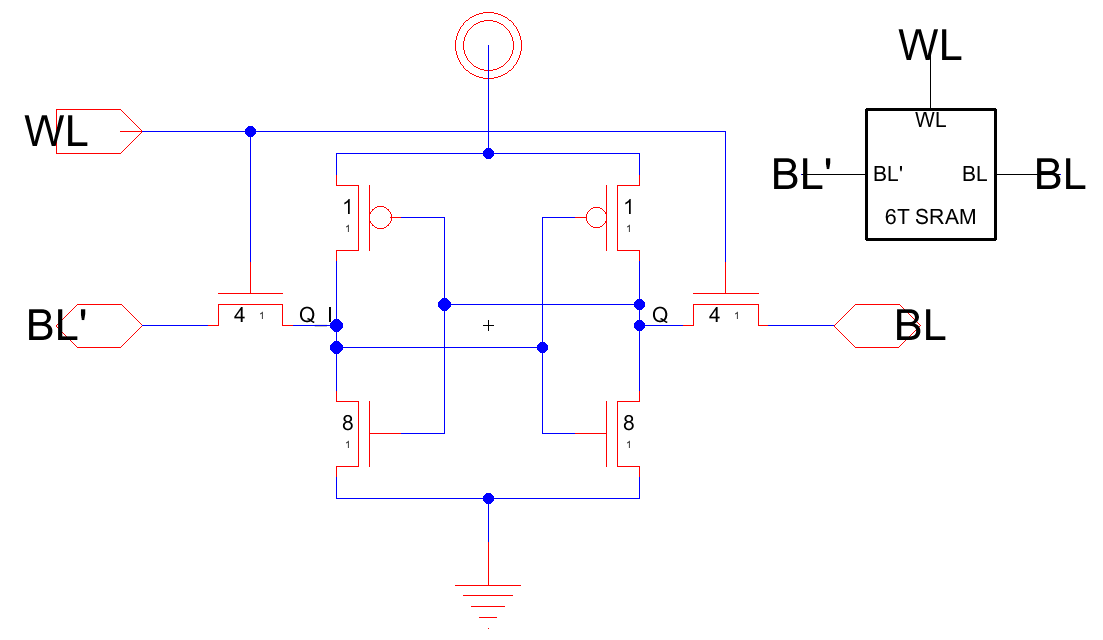
\includegraphics[width=1.0\textwidth]{sram_cell_circuit.PNG}
  \caption{Sized SRAM memory cell circuit}
  \label{fig:sram_cell_circuit}
\end{figure}

\subsection*{Tri-State Buffer Schematic}
\begin{figure}[H]
  \centering
    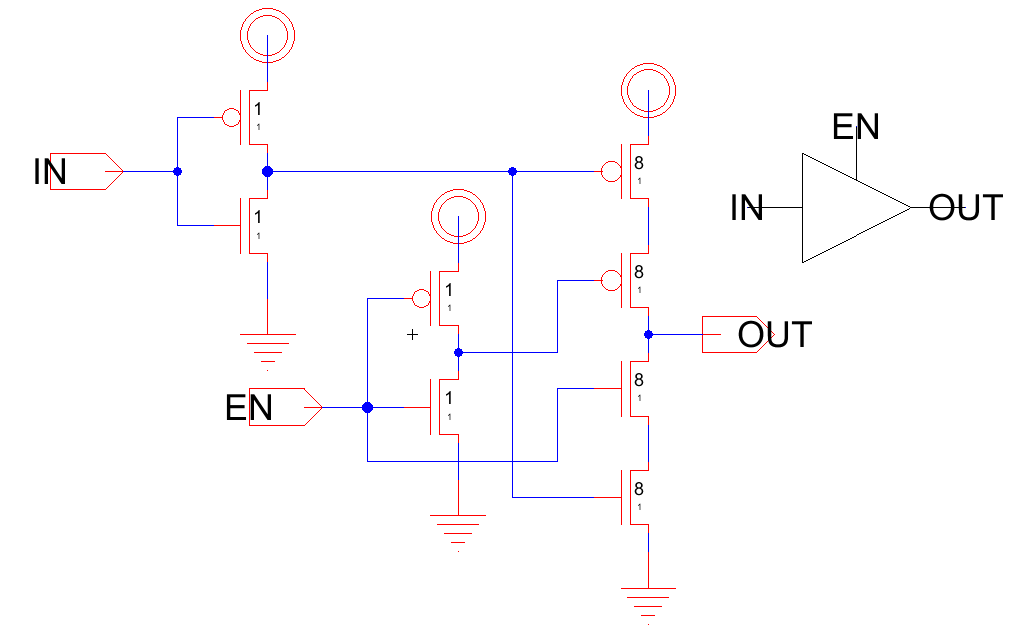
\includegraphics[width=1.0\textwidth]{tristate_buffer_circuit.PNG}
  \caption{Tri-state buffer circuit}
  \label{fig:tristate_buffer_circuit}
\end{figure}

\subsection*{Tri-State Inverter Schematic}
\begin{figure}[H]
  \centering
    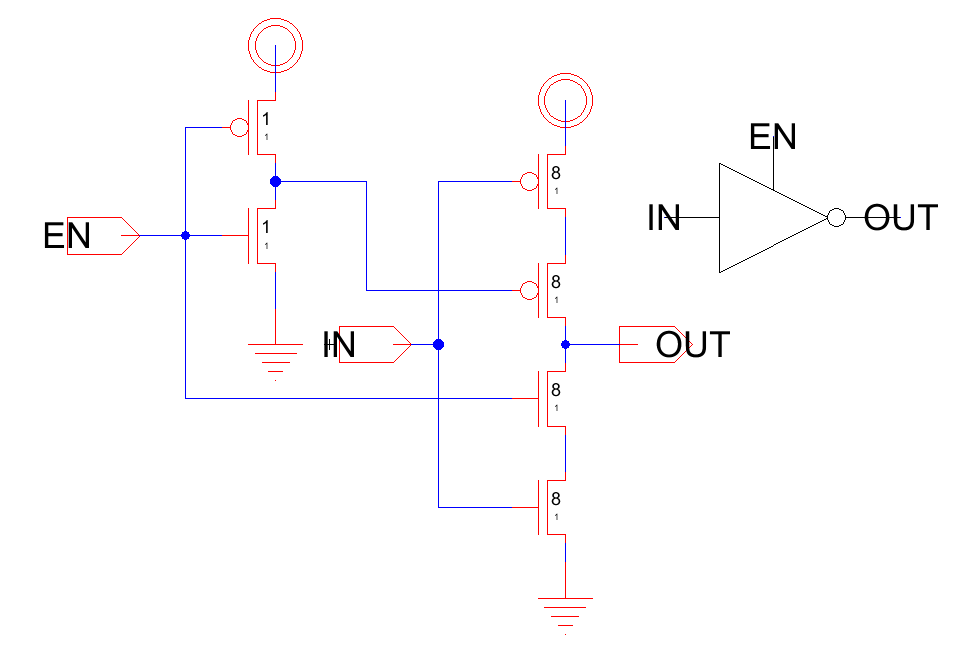
\includegraphics[width=1.0\textwidth]{tristate_inverter_circuit.PNG}
  \caption{Tri-state inverter circuit}
  \label{fig:tristate_inverter_circuit}
\end{figure}


\section*{Reading and Writing (Cell)}
\subsection*{Test Cases to Consider}
For writing to the cell, we considered four cases:
\begin{enumerate}
\item Writing a 0 to a cell with 0 (Figure \ref{fig:write_0_then_write_0}). We first write a 0 by driving $BL$ low and $BL'$ high by driving $write\_enable$ high, and driving $WL$ to high. We then write a 0 again using the same process. The $Q$ and $Q'$ signals inside the cell were verified to ensure that writes were being completed properly, even after $write_enable$ was set low.
\item Writing a 1 to a cell with 0 (Figure \ref{fig:write_0_then_write_1}). This uses the same process for writing a 1 as for writing a 0, but $BL$ is driven high and $BL'$ is driven low.
\item Writing a 0 to a cell with 1 (Figure \ref{fig:write_1_then_write_0}). Since the cell already starts in a state in which $Q$ is high and $Q'$ is low, we only need to write a 1 to verify this case.
\item Writing a 1 to a cell with 1 (Figure \ref{fig:write_1_then_write_1}). This is the same case as (3) in that the cell already starts with $Q = 1$, but we instead write a 1.
\end{enumerate}

Since there are two present states ($Q_t = 0$, $Q_t = 1$) and two next states ($Q_{t+1} = 0$, $Q_{t+1} = 1$), these four cases completely test writing to the cell.

For reading from the cell, we considered two cases:
\begin{enumerate}
\item Reading a 0 from a cell that was written to 0 (Figure \ref{fig:write_0_then_read_0}).
\item Reading a 1 from a cell that was written to 1 (Figure \ref{fig:write_1_then_read_1}).
\end{enumerate}

In each reading case, we made sure that the reading process did not cause enough of a read upset to overwrite $Q$. These read upsets are not visible in Figures \ref{fig:write_0_then_read_0} or \ref{fig:write_1_then_read_1} and were on the order of tens of millivolts, so we are confident that reading from these cells is not destructive.

All testing was done with the test circuit in Figure \ref{fig:test_circuit}. Note that this test circuit includes only one SRAM cell to keep the image visible. Actual testing was done on one SRAM cell with 15 other SRAM cells loading the bitlines in parallel to simulate how the memory circuit would behave in the actual 16-word FIFO queue.

\begin{figure}[H]
  \centering
    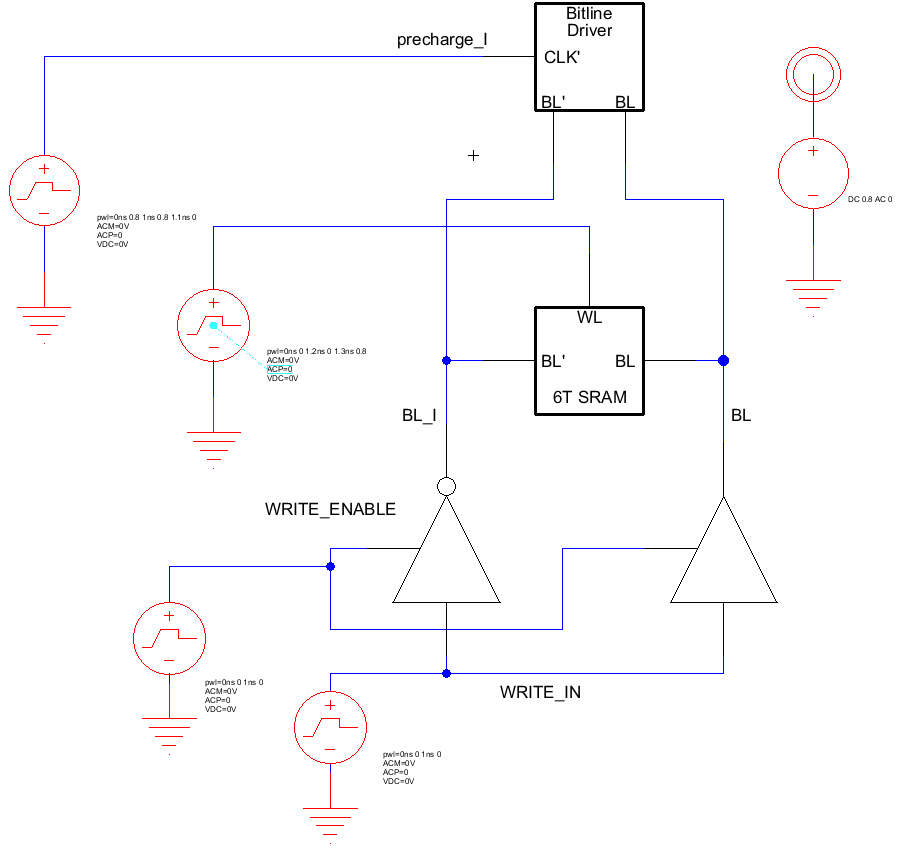
\includegraphics[width=1.0\textwidth]{test_circuit.PNG}
  \caption{Memory cell test circuit}
  \label{fig:test_circuit}
\end{figure}

\subsection*{SRAM Cell Test Results}
\begin{figure}[H]
  \centering
    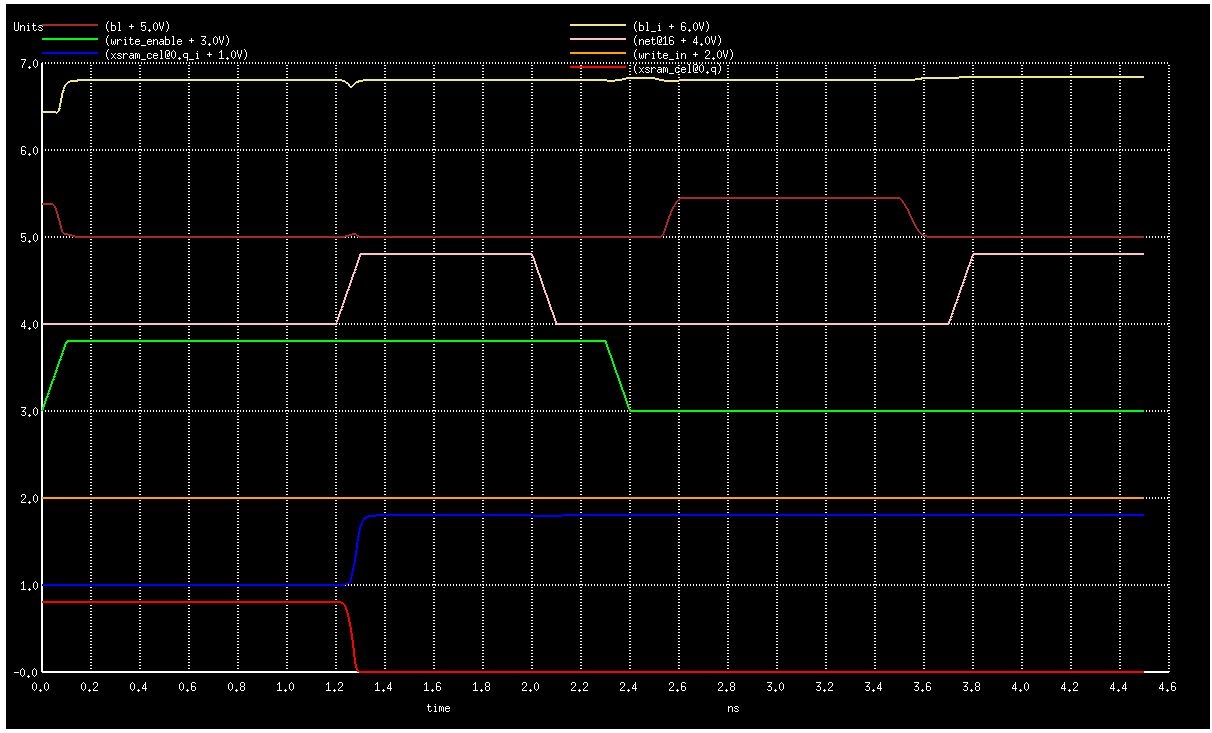
\includegraphics[width=1.0\textwidth]{write_0_then_read_0.png}
  \caption{Writing 0 and then reading 0}
  \label{fig:write_0_then_read_0}
\end{figure}

\begin{figure}[H]
  \centering
    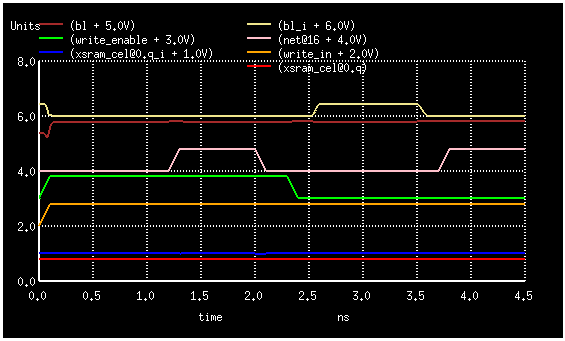
\includegraphics[width=1.0\textwidth]{write_1_then_read_1.png}
  \caption{Writing 1 and then reading 1}
  \label{fig:write_1_then_read_1}
\end{figure}

\begin{figure}[H]
  \centering
    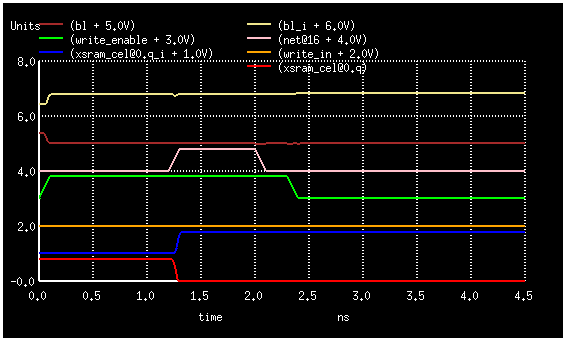
\includegraphics[width=1.0\textwidth]{write_1_then_write_0.png}
  \caption{Writing 0}
  \label{fig:write_1_then_write_0}
\end{figure}

\begin{figure}[H]
  \centering
    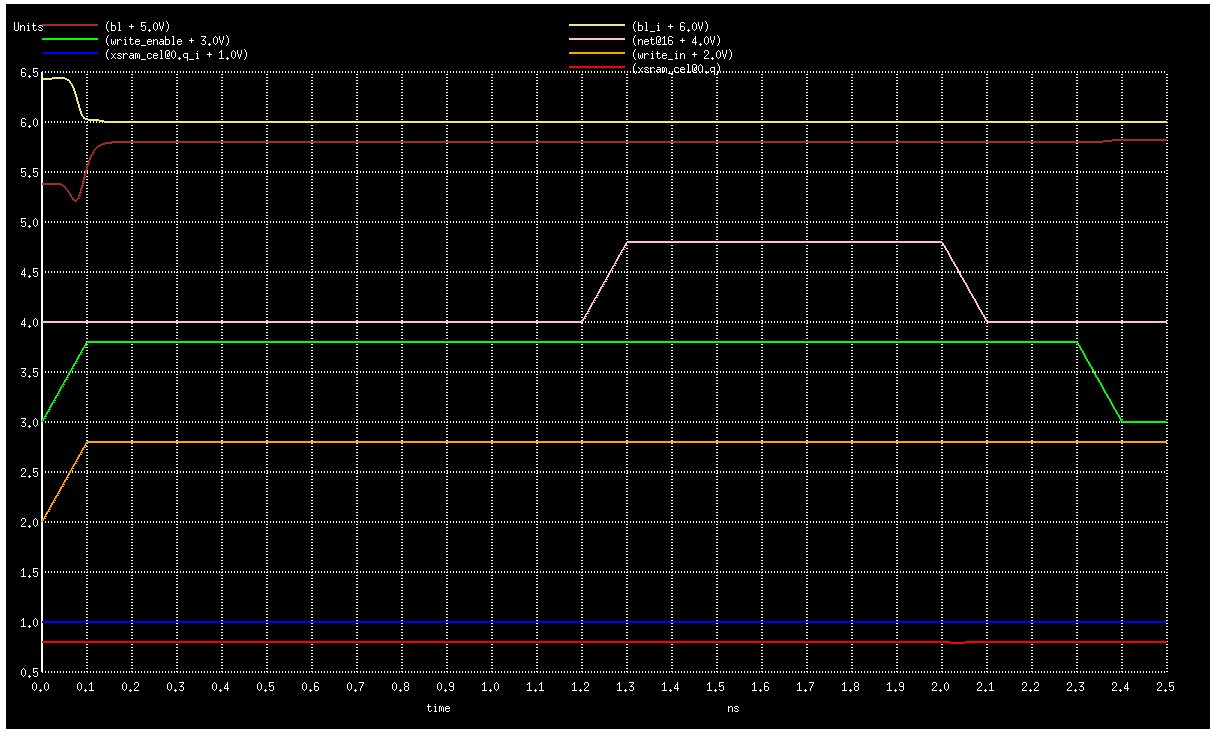
\includegraphics[width=1.0\textwidth]{write_1_then_write_1.png}
  \caption{Writing 1}
  \label{fig:write_1_then_write_1}
\end{figure}

\begin{figure}[H]
  \centering
    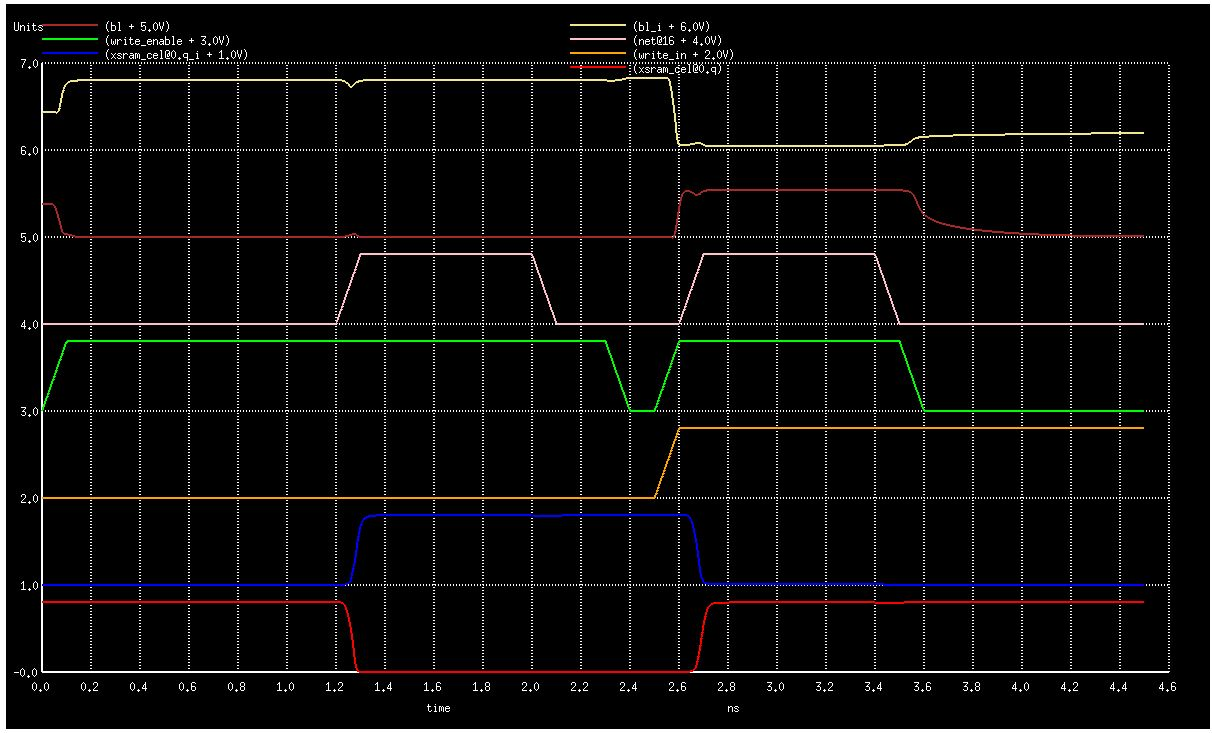
\includegraphics[width=1.0\textwidth]{write_0_then_write_1.png}
  \caption{Writing 0, then writing 1}
  \label{fig:write_0_then_write_1}
\end{figure}

\begin{figure}[H]
  \centering
    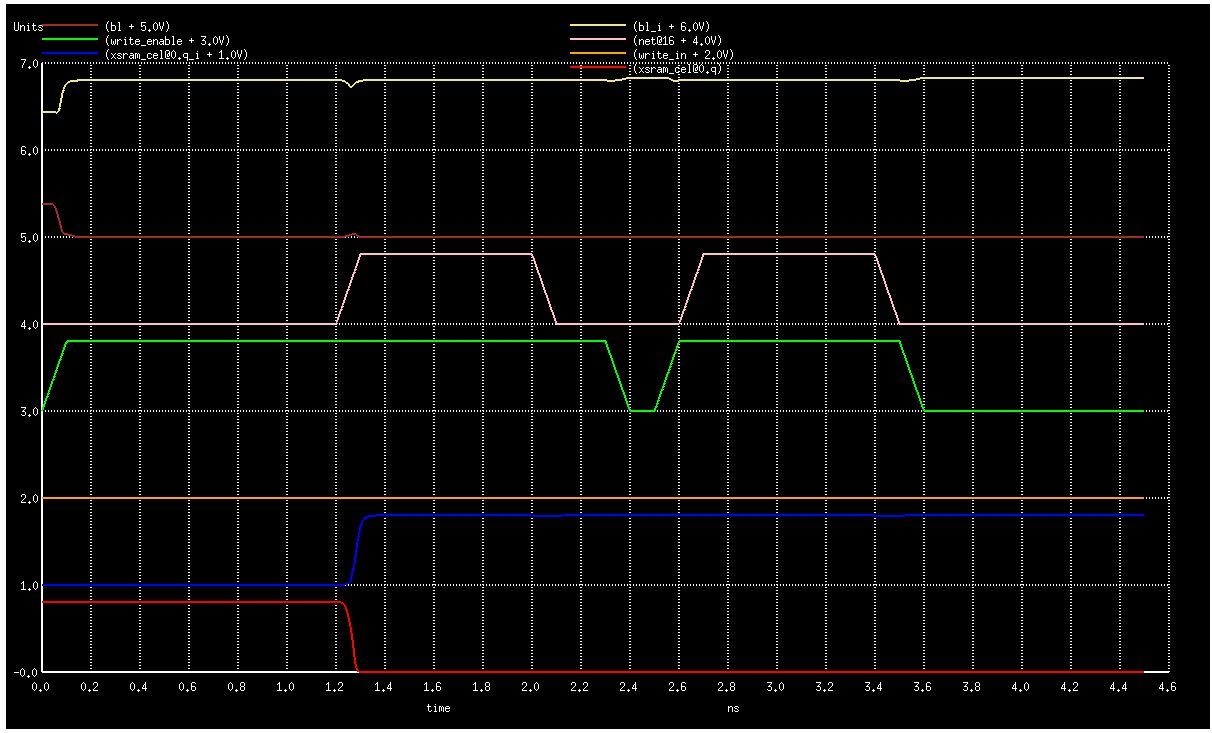
\includegraphics[width=1.0\textwidth]{write_0_then_write_0.png}
  \caption{Writing 0, then writing 0}
  \label{fig:write_0_then_write_0}
\end{figure}

\section*{Constraints on Write Timing, Full FIFO Design}
One important constraint for write timing is if we are simultaneously enqueuing and dequeuing from the same word at the same time. To ensure that the dequeue operation returns the correct value to the output, and because a cell can only be written to or read in a single clock cycle, we will want to make sure that we dequeue the old value first before enqueueing the new value. To test this, we will first enqueue a single element (suppose it's "0011"), and then we'll issue both an enqueue (say, of "1100") and a dequeue at the same time. The value returned by dequeue should be "0011".
\end{document}
